\section{My First Plot}

\begin{figure}
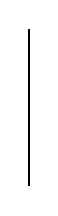
\begin{tikzpicture}
 \draw[thick,rounded corners=18pt]
(0,0) -- (0,2);    %  -- (1,3.25) -- (2,2) -- (2,0) -- (0,2) -- (2,2) -- (0,0) -- (2,0);
\end{tikzpicture}
\caption{You can draw lines of various thicknesses with tikz by using key value parameters.}
\end{figure}

The path starts at 0,0 the origin. You then continue from there.
\begin{figure}
\begin{tikzpicture}
 \draw[thick]
(0,0) -- (0,2)  -- (2,2);% -- (2,2) -- (2,0) -- (0,2) -- (2,2) -- (0,0) -- (2,0);
\end{tikzpicture}
\caption{You can draw lines of various thicknesses with tikz by using key value parameters.}
\end{figure}

We can draw an arrow by utilizing another style.
The path starts at 0,0 the origin. You then continue from there.
\begin{figure}
\begin{tikzpicture}
 \draw[->, thick]
(0,0) -- (0,2)  -- (2,2);% -- (2,2) -- (2,0) -- (0,2) -- (2,2) -- (0,0) -- (2,0);
\end{tikzpicture}
\caption{You can draw lines of various thicknesses with tikz by using key value parameters.}
\end{figure}


\section{Clipping}
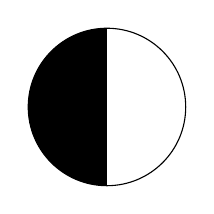
\begin{tikzpicture}
\draw (0,0) circle (1cm);
\clip (0,0) circle (1cm);
\fill[black] (0cm,1cm) rectangle (-1cm,-1cm);
\end{tikzpicture}




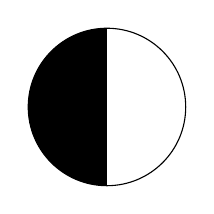
\begin{tikzpicture}
\draw (0,0) circle (1cm);
\clip (0,0) circle (1cm);
\fill[black] (0cm,1cm) rectangle (-1cm,-1cm);
\end{tikzpicture}


\section{Beyond line segments}

In addition to points and line segments, there are a number of other graphic
primitives available. These include:

\begin{enumerate}
\item  Grids and rectangles
\item Circles and ellipses
\item  Arcs
\item  Bézier curves
\end{enumerate}

As previously discussed, a grid is specified by providing two diagonally opposing
points and other options which affect such things as the color and spacing of the
grid lines. A rectangle can be viewed as a simplified grid — all that is needed are
two diagonally opposing points of the rectangle. The syntax

backslash draw (P) rectangle (Q);

draws the rectangle specified by the two “bounding box” points P and Q. It is
worth noting that the current point is updated to Q, a fact which plays a role if
the backslash draw command involves more than one drawing action. Figure 14 provides
an example where three rectangles are drawn in succession. Each rectangle operation
updates the current point, which then serves as one of the bounding box
points for the following rectangle.

\begin{tikzpicture}
\draw [color=magenta](0,0) rectangle (1,1)
rectangle (3,2)
rectangle (4,3);
\end{tikzpicture}

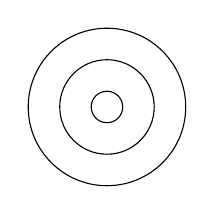
\begin{tikzpicture}
\draw (0,0) circle (1cm)
circle (0.6cm)
circle (0.2cm);
\end{tikzpicture}


\subsection{arcs}

Arcs are drawin in degrees, remember -- denotes a straight line, but in this case it rather denotes a connection.
\begin{verbatim}
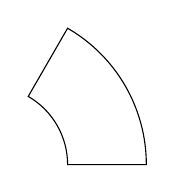
\begin{tikzpicture}
\draw (0:1cm) -- (0:2cm)
arc (0:60:2cm) -- (60:1cm)
arc (60:0:1cm) -- cycle;
\end{tikzpicture}
\end{verbatim}

By using arc, we can generate arcs rather than circles. This can be quite useful.

\begin{figure}
\begin{center}
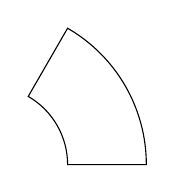
\begin{tikzpicture}
\draw (0:1cm) -- (0:2cm)
arc (0:60:2cm) -- (60:1cm)
arc (60:0:1cm) -- cycle;
\end{tikzpicture}
\caption{An arc drawn in a counterclock fashion}
\end{center}
\end{figure}

We can color the figure by using {\tt color=magenta}.

\begin{figure}
\begin{center}
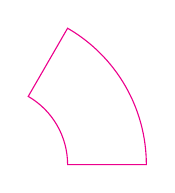
\begin{tikzpicture}
\draw[color = magenta] (0:1cm) -- (0:2cm)
arc (0:60:2cm) -- (60:1cm)
arc (60:0:1cm) -- cycle;
\end{tikzpicture}
\caption{An arc drawn in a counterclock fashion}
\end{center}
\end{figure}

\section{From coordinates to nodes}

A node is a generalization of the coordinate primitive. Two characteristics of a
node are its shape and its text. A node allows for arbitrary TEX text to appear
within a diagram. The command


defines a node named v0, centered at the origin, with a circular shape and text
component $v_0$. The draw option causes the associated shape (in this case, a
circle) to be drawn. Figure 24 illustrates how nodes can be used to draw an undirected
graph. Notice how line segments which join nodes stop at the boundary

\begin{marginfigure}[5cm]
\begin{verbatim}
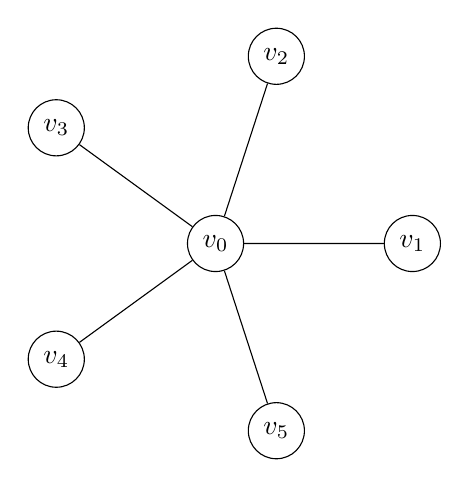
\begin{tikzpicture}[scale=2.5]
\tikzstyle{every node}=[draw,shape=circle];
\path (0:0cm) node (v0) {$v_0$};
\path (0:1cm) node (v1) {$v_1$};
\path (72:1cm) node (v2) {$v_2$};
\path (2*72:1cm) node (v3) {$v_3$};
\path (3*72:1cm) node (v4) {$v_4$};
\path (4*72:1cm) node (v5) {$v_5$};
\draw (v0) -- (v1)
(v0) -- (v2)
(v0) -- (v3)
(v0) -- (v4)
(v0) -- (v5);
\end{tikzpicture}
\end{verbatim}
\end{marginfigure}


\begin{center}
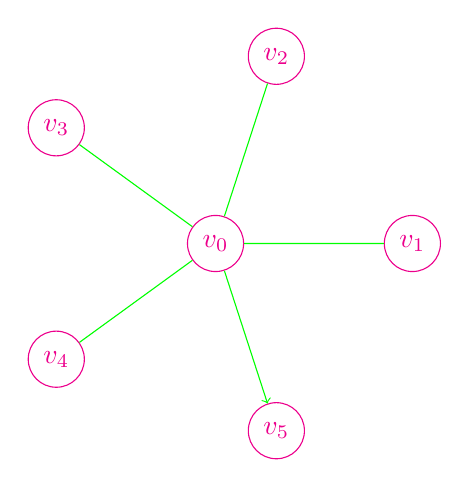
\begin{tikzpicture}[scale=2.5]
\tikzstyle{every node}=[draw,shape=circle, color=magenta];
\path (0:0cm) node (v0) {$v_0$};
\path (0:1cm) node (v1) {$v_1$};
\path (72:1cm) node (v2) {$v_2$};
\path (2*72:1cm) node (v3) {$v_3$};
\path [color=green] (3*72:1cm) node (v4) {$v_4$};
\path (4*72:1cm) node (v5) {$v_5$};
\draw [->, color=green] (v0) -- (v1)
(v0) -- (v2)
(v0) -- (v3)
(v0) -- (v4)
(v0) -- (v5);
\end{tikzpicture}
\end{center}


TikZ introduces a special syntax for adding text or, more generally, nodes to a graphic. When you specify
a path, add nodes as in the following example:
text

\begin{verbatim} \tikz \draw (1,1) node {text} -- (2,2); \end{verbatim}

Nodes are inserted at the current position of the path, but only after the path has been rendered. When
special options are given, as in draw (1,1) node[circle,draw] {text};, the text is not just put at the
current position. Rather, it is surrounded by a circle and this circle is "drawn."

You can add a name to a node for later reference either by using the option name=hnode namei or by
stating the node name in parentheses outside the text as in node[circle](name){text}.

Predefined shapes include rectangle, circle, and ellipse, but it is possible (though a bit challenging)
to define new shapes.

\section{Special Syntax for Specifying Trees}

In addition to the "node syntax,"  TikZ also introduces a special syntax for drawing trees. The syntax is
intergrated with the special node syntax and only few new commands need to be remebered. In essence, a
node can be followed by any number of children, each introduced by the keyword child. The children are
nodes themselves, each of which may have children in turn.
\begin{marginfigure}
\begin{verbatim}
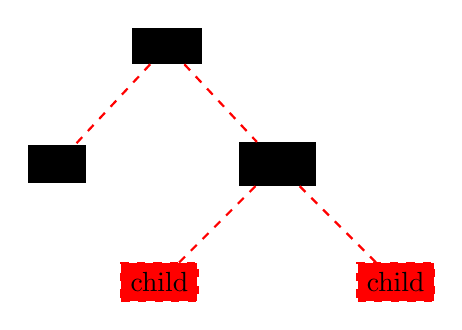
\begin{tikzpicture}
\node {root}
child {node {left}}
child {node {right}
child {node {child}}
child {node {child}}
};
\end{tikzpicture}
\end{verbatim}
\end{marginfigure}


\begin{figure}
\begin{center}
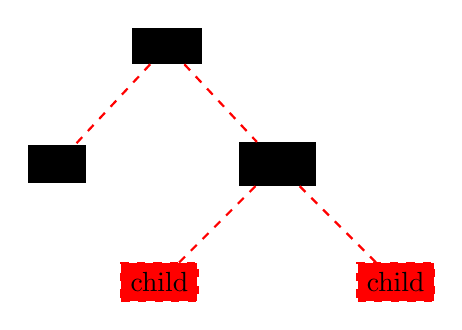
\begin{tikzpicture}
\node {root}
child {node {left}}
child {node {right}
child {node {child}}
child {node {child}}
};
\end{tikzpicture}
\end{center}
\end{figure}
Since trees are made up from nodes, it is possible to use options to modify the way trees are drawn. Here
are two examples of the above tree, redrawn with different options:

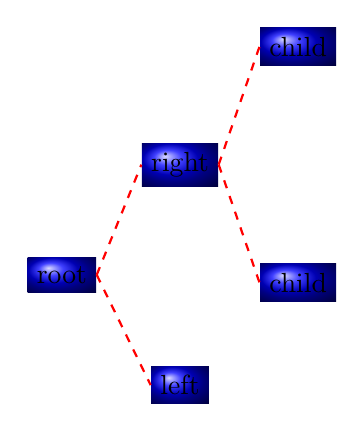
\begin{tikzpicture}
[parent anchor=east,child anchor=west,grow=east]
\tikzstyle{every node}=[ball color=blue, rectangle, text=black]
\tikzstyle{edge from parent}=[draw,dashed,thick,red]
\node {root}
child {node {left}}
child {node {right}
child {node {child}}
child {node {child}}
};
\end{tikzpicture}


Shading is accomplished by a style \tikz \shadedraw [shading=axis,shading angle=90] (0,0) rectangle (1,1);

\begin{figure}
\begin{center}
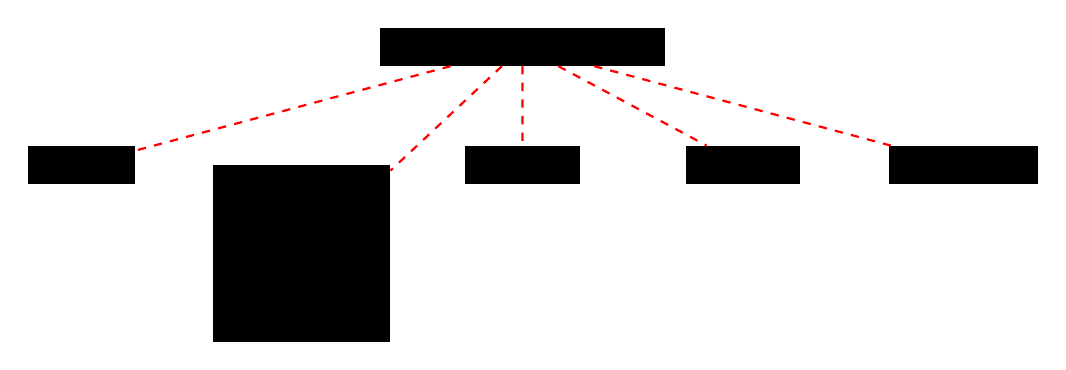
\begin{tikzpicture}

\tikzstyle{level 1}=[sibling distance=28mm]
\tikzstyle{level 2}=[sibling distance=30mm]
\tikzstyle{level 3}=[sibling distance=30mm]

\node {Construction Director}
child {node { Rotana}}
child {node [text width=2cm, anchor=north]{\bf Shangrila and other bold matters of importance}}
child{node {Merweb}}
child{node{Podium}}
child{node{Planrooms}};
\end{tikzpicture}
\end{center}
\end{figure}
\newpage

\chapter{Repeating Things}
\small
TikZ provides a loop structure which can simplify the creation of certain types of
graphics. The basic loop syntax is as follows:

\begin{verbatim}
\foreach \var in {iteration list}
   {
      loop body
    }
\end{verbatim}

The loop variable, {{\tt var}}, takes on the values given in the iteration list. In the
simplest case, this list can be a fixed list of values, such as {1,2,3,4} or as an
implied list of values, such as {1,...,4}.

Consider the loop in Figure 26. Four coordinates, X1 through X4 are introduced
at (1, 0), (2, 0), (3, 0), and (4, 0), respectively. In addition, a small filled
circle is drawn at each coordinate.

Figure 27 shows how to extend this idea to yield a bipartite graph. As one
might expect, foreach loops can be nested, a feature utilized here to specify all
the edges in the graph.

Iteration lists need not consist of consecutive integers. An implicit step size is
obtained by providing the first two values of the list in addition to the final value.






another test
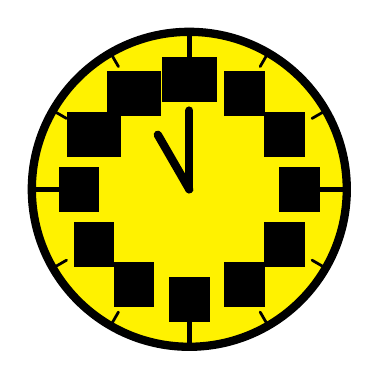
\begin{tikzpicture}[cap=round,line width=3pt]
\filldraw [fill=yellow] (0,0) circle (2cm);
\foreach \angle / \label in
{0/3, 30/2, 60/1, 90/12, 120/11, 150/10, 180/9,
210/8, 240/7, 270/6, 300/5, 330/4}
{
\draw[line width=1pt] (\angle:1.8cm) -- (\angle:2cm);
\draw (\angle:1.4cm) node{\textsf{\label}};
}
\foreach \angle in {0,90,180,270}
\draw[line width=2pt] (\angle:1.6cm) -- (\angle:2cm);
\draw (0,0) -- (120:0.8cm); % hour
\draw (0,0) -- (90:1cm); % minute
\end{tikzpicture}%

\tikz \fill[fill=yellow]
(0,0) node {first node}
-- (1,1) node  {second node}
-- (0,2) node {third node};

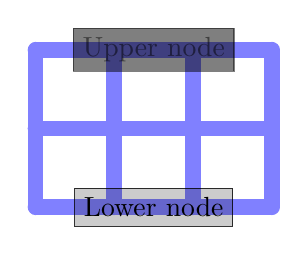
\begin{tikzpicture}
\draw[line width=2mm,blue!50,cap=round] (0,0) grid (3,2);
\tikzstyle{every node}=[fill,draw]
\node[opacity=0.5] at (1.5,2) {Upper node};
\node[draw opacity=0.8,fill opacity=0.2,text opacity=1]
at (1.5,0) {Lower node};
\end{tikzpicture}

\chapter{Paths}

\begin{pgfpicture}
\pgfpathmoveto{\pgfpointorigin}
\pgfpathlineto{\pgfpoint{1cm}{1cm}}
\pgfpathlineto{\pgfpoint{2cm}{1cm}}
\pgfpathlineto{\pgfpoint{3cm}{0.5cm}}
\pgfpathlineto{\pgfpoint{3cm}{0cm}}
\pgfsetfillcolor{red}
\pgfusepath{fill,stroke}
\end{pgfpicture}

check this one out for a while 


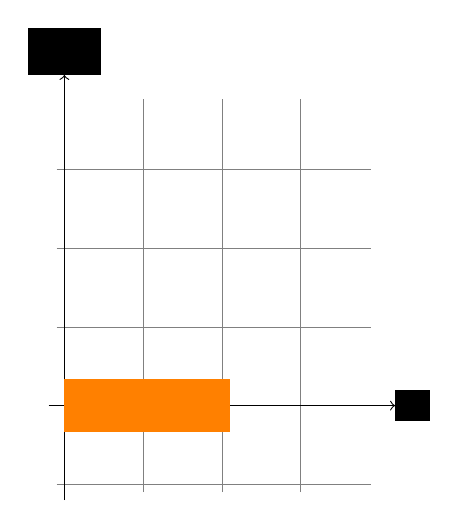
\begin{tikzpicture}[domain=0:4]
\draw[very thin,color=gray] (-0.1,-1.1) grid (3.9,3.9);
\draw[->] (-0.2,0) -- (4.2,0) node[right] {$x$};
\draw[->] (0,-1.2) -- (0,4.2) node[above] {$f(x)$};
\draw[color=red] plot[id=x] function{x} node[right] {$f(x) =x$};
\draw[color=blue] plot[id=sin] function{sin(x)} node[right] {$f(x) = \sin x$};
\draw[color=orange] plot[id=exp] function{0.05*exp(x)} node[right] {$f(x) = \frac{1}{20} \mathrm e^x$};
\end{tikzpicture}




 \chapter{Plotting}
\begin{figure}
% Preamble: \pgfplotsset{width=7cm,compat=1.3}
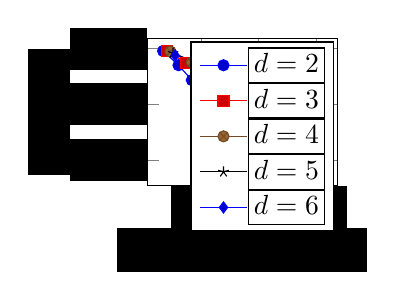
\begin{tikzpicture}
\begin{loglogaxis}[
xlabel={Degrees of freedom},
ylabel={$L_2$ Error}
]
\addplot coordinates {
(5,8.312e-02) (17,2.547e-02) (49,7.407e-03)
(129,2.102e-03) (321,5.874e-04) (769,1.623e-04)
(1793,4.442e-05) (4097,1.207e-05) (9217,3.261e-06)
};
\addplot coordinates{
(7,8.472e-02) (31,3.044e-02) (111,1.022e-02)
(351,3.303e-03) (1023,1.039e-03) (2815,3.196e-04)
(7423,9.658e-05) (18943,2.873e-05) (47103,8.437e-06)
};
\addplot coordinates{
(9,7.881e-02) (49,3.243e-02) (209,1.232e-02)
(769,4.454e-03) (2561,1.551e-03) (7937,5.236e-04)
(23297,1.723e-04) (65537,5.545e-05) (178177,1.751e-05)
};
\addplot coordinates{
(11,6.887e-02) (71,3.177e-02) (351,1.341e-02)
(1471,5.334e-03) (5503,2.027e-03) (18943,7.415e-04)
(61183,2.628e-04) (187903,9.063e-05) (553983,3.053e-05)
};
\addplot coordinates{
(13,5.755e-02) (97,2.925e-02) (545,1.351e-02)
(2561,5.842e-03) (10625,2.397e-03) (40193,9.414e-04)
(141569,3.564e-04) (471041,1.308e-04) (1496065,4.670e-05)
};
\legend{$d=2$,$d=3$,$d=4$,$d=5$,$d=6$}
\end{loglogaxis}

\end{tikzpicture}
\caption{A multiline graph}
\end{figure}

The beauty of this package is that we can use equations for plotting.


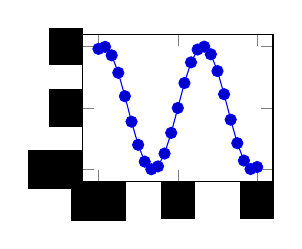
\begin{tikzpicture}
\begin{axis}
\addplot {sin(deg(x))};
\end{axis}
\end{tikzpicture}


\noindent We can draw two graphs one on top of each other by using some text in between. this will force \LaTeXe to float the figures better.


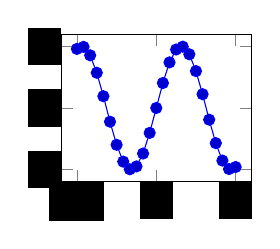
\begin{tikzpicture}
\begin{axis}
\addplot {sin(deg(x))+2}; %the + will only use the points
\end{axis}
\end{tikzpicture}

Using the Tufte book package we can place figures in the margin as well. This is very good.
\begin{marginfigure}
\pgfplotsset{width=4cm,compat=1.3}
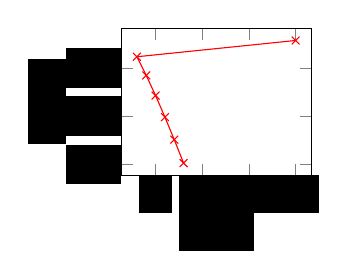
\begin{tikzpicture}
\begin{axis}[
xlabel=Cost,
ylabel=Error]
\addplot[color=red,mark=x] coordinates {
(20,-2.8559703)
(3,-3.5301677)
(4,-4.3050655)
(5,-5.1413136)
(6,-6.0322865)
(7,-6.9675052)
(8,-7.9377747)
};
\end{axis}
\end{tikzpicture}
\end{marginfigure}

\begin{center}
\color{brown}{
\small{
\begin{verbatim}
           %\usepackage{ifthen}
          \newcommand{\weekday}[1]%
         {%
             \ifthenelse{\equal{#1}{1}}{Monday}{}%
             \ifthenelse{\equal{#1}{2}}{Tuesday}{}%
             \ifthenelse{\equal{#1}{3}}{Wednesday}{}%
             \ifthenelse{\equal{#1}{4}}{Thursday}{}%
             \ifthenelse{\equal{#1}{5}}{Friday}{}%
             \ifthenelse{\equal{#1}{6}}{Saturday}{}%
             \ifthenelse{\equal{#1}{7}}{Sunday}{}%
}

\weekday{3}

\end{verbatim}
}
}
\end{center}

\begin{tabular}{|lll}
\toprule
sl. & item & price\\
\midrule
1  & Butterfly valves & 23\\
\bottomrule
\end{tabular}




